
\chapter{PickCell: from image analysis to physical simulation} 
 
{\sl The associated software is available in the Pickcell package pn Store at http://wsn.univ-brest.fr.
Use is similar to  chapter  \ref{sec:chapter5bis} explanations: 
\begin{itemize}
\item load pickcell, then load a file image from the application window seleted from Tool menu,
\item load quickmap, then select the quickmap pickcell variant from tool menu, to enable
pickcell from an OpenStreetMap view.
\end{itemize}
}


Creation of sensing machines working in the environment necessitate 
a validation  in the context of physical scenarios. Some of these 
scenario are flooding, insect clouds, pollutions, fires.

The focus of this chapter are tools and methods allowing to produce inputs and  organizations
for physical  simulations. These simulation involve lot of computations. A  choice
is to use  space and time  discrete  models such as
cellular automata. It is also expected that physical simulation  will cooperate with network simulations
in various ways: production of stimuli on sensors, or  modificaton  of the sensor network 
itself. Figure \ref{fig:physics+sensorsFlow} displays the general scenario with
the left branch being discussed here.



\begin{figure}[hbtp]
\begin{center} 
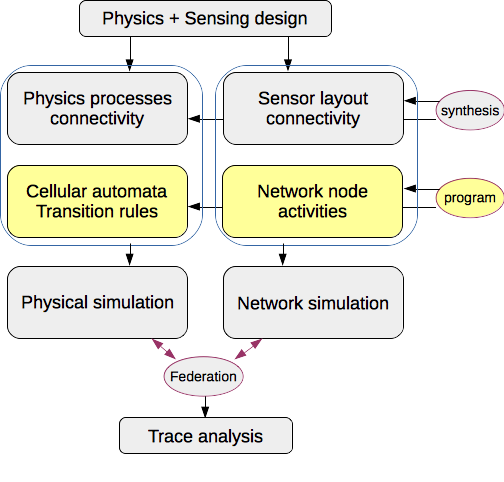
\includegraphics[width=8cm]{physics+sensorsFlow.png}
\caption{General flow for simulation with the physical simulation and the network simulation.
Both share coordination  informations such as geographical or geometrical points, clocking system,
and they can be coordinated during the simulation.}
\label{fig:physics+sensorsFlow}
\end{center}
\end{figure}


The interest of image anlysis is to  produce sets of  regions that share similar characteristics.
Analysis follows a conventional flow, starting from a picture coming  from
photographies, maps, radar images, to obtain regions of interests, on which physical simulation  will
take place.

\begin{figure}[hbtp]
\begin{center} 
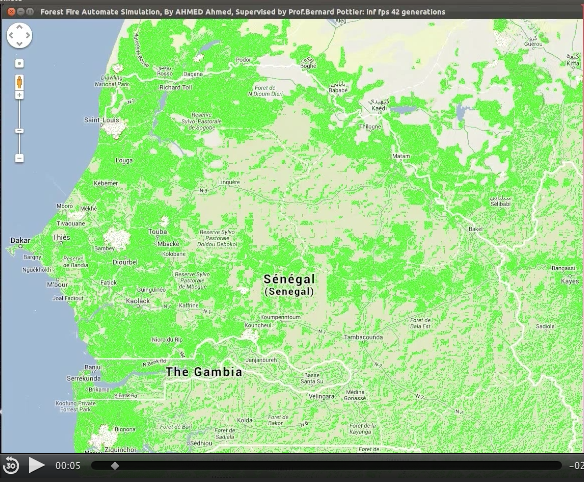
\includegraphics[width=10cm]{AhmedFire.png}
\caption{Example of a fire simulation  using Cellular Automata  cells that have  states such as:
vegetation, burning, ashes.}
\label{fig:AhmedFire}
\end{center}
\end{figure}

A reference for processing on such regions are cellular automata
reproducing fire expansions of phenomenon consuming  vegetation.
Figure \ref{fig:AhmedFire} is extracted from a
movie demonstration where "fires" are started randomly to "eat" such vegetation report \cite{AhmedFire}. This
preliminary work was achieved on an Nvidia GPU.

The chapter will provide details on the production of   systems representing the physical
process working in harmony with the sensing systems.

\section{Image processing  flow for cellular system synthesis}

Thus,   modeling  physical regions automatically, or semi-automatically, following physical process 
characteristics, is certainly critical to lead both physical and control network  simulations jointly,
and synchronously. One can think of this as a sampling technique of the physical process sharing
a clock with the sensing network. Cellular automata are one way to implement the real world simulation,
starting from initial states and regions.


A general flow to obtain such regions  is  shown figure \ref{fig:pickcellFlow}~:
\begin{enumerate}
\item  preprocessing  images 
\item segmenting images into blocks
\item recognition of similar cells and grouping into regions
\item processing regions an obtaining skeleton images
\end{enumerate}

\begin{figure}[hbtp]
\begin{center} 
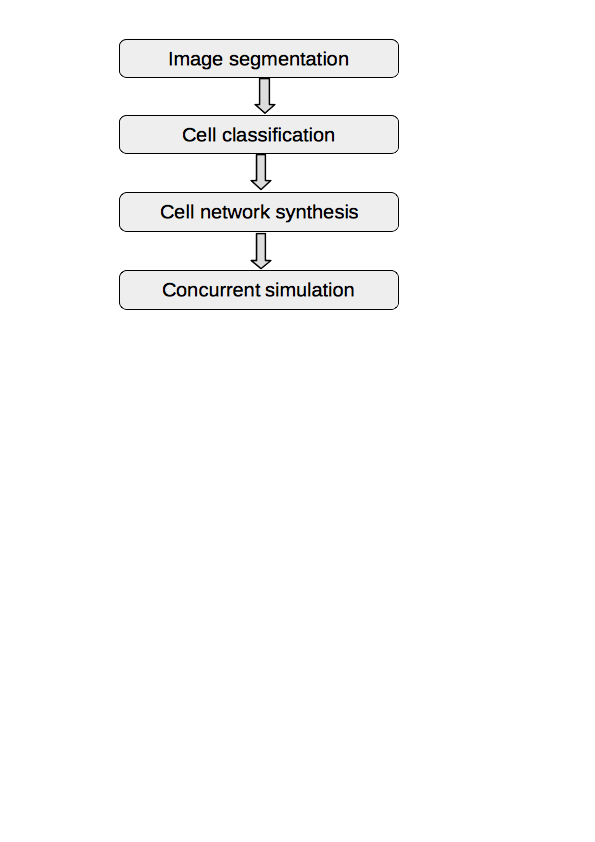
\includegraphics[width=6cm]{pickcellFlow.png}
\caption{Preparing cellular automata from image analysis: synthesis flow.}
\label{fig:pickcellFlow}
\end{center}
\end{figure}

Following this flow, higher level objects can be obtained, still with geographical definition in the case of
maps, or satellite imagery.

\subsection {Preprocessing for image preparation }

In the case of maps, geographic information is yet presented in a comprehensive way. However analyzing maps is still useful
to obtain information without the direct contact of an initial information system (GIS).
More difficult is the case of satellite or air  images, because the synthesis of objects necessitate
pre processing. Figure \ref{fig:sideBySide} shows an example of procesing achieved using common tools
for management of photographies. The initial view is a satellite image (left), while the right part displays an improved
view, with better contrasts.

\begin{figure}[hbtp]
\begin{center} 
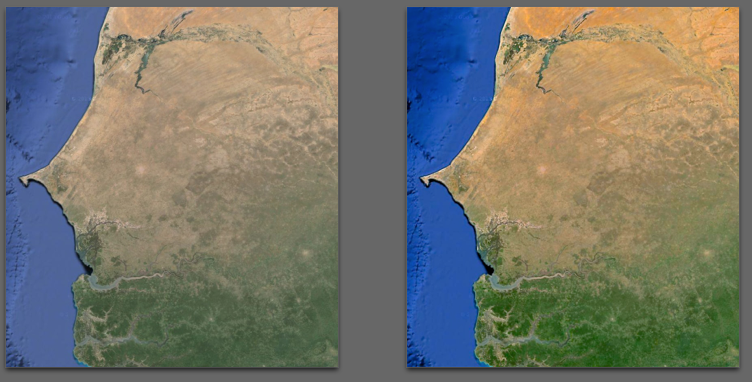
\includegraphics[width=10cm]{SenegalSideBySide.png}
\caption{Modifying original image for better contrasts or coulour selections. Image is a satellite view from Google Maps.}
\label{fig:sideBySide}
\end{center}
\end{figure}

These representations are coming from a very common image processing software 
allowing to change contrasts and colour mapping to fit tne necessity of the recognition.
Image processing paramers show the Red Green Blue statistic values in the original
and the modified image, with a better use of the value range in the second case
(Figure \ref{fig:colours1+2}).



\begin{figure}[hbtp]
\begin{center}
\leavevmode 
\begin{minipage}{6cm}
\begin{center} 
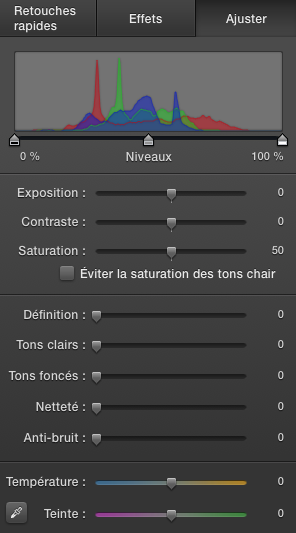
\includegraphics[width=6cm]{senegalColours.png} 
\end{center}
\end{minipage}~~~~~~~~~\begin{minipage}{6cm}
\begin{center} 
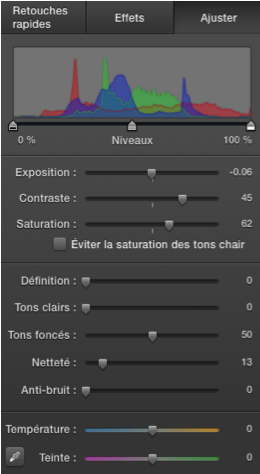
\includegraphics[width=6cm]{senegalColours2.png} 
\end{center}
\end{minipage}
\caption{RGB colour statistics for the left original picture, and its adaptation (right). The software
is Apple iPhoto, standard to any MacOs computer. Similar functions could be obtained from Linux GIMP,
and probably reimplemented from a Palette tool in NetGen.}
\label{fig:colours1+2}
\end{center}
\end{figure}
  
\subsection { Segmenting the image into cells}

To obtain regions, it is necessary to group zones of the image based on similarities of different kind.
The first operation is a fragmentation into blocks of different size and geometry. Of course,
squares, or rectangles are the simplest way to proceed, but other fragmentation techniques could also
be suitable and ease further stages in simulation. Cellular automata propose as example  an hexagonal
shape where each cell has 6 direct neighbours.

{\sc PickCell} has been implemented     to ease this fragmentation, in relation with 
further networks synthesis operations.

This tool reuse the {\sl Picking} framework presented Figure  \ref{fig:PickPoint1}. Beside the capability
to load images, and specify sensor positions, there is the ability to install a rectangular grid over the
image.


\begin{figure}[hbtp]
\begin{center} 
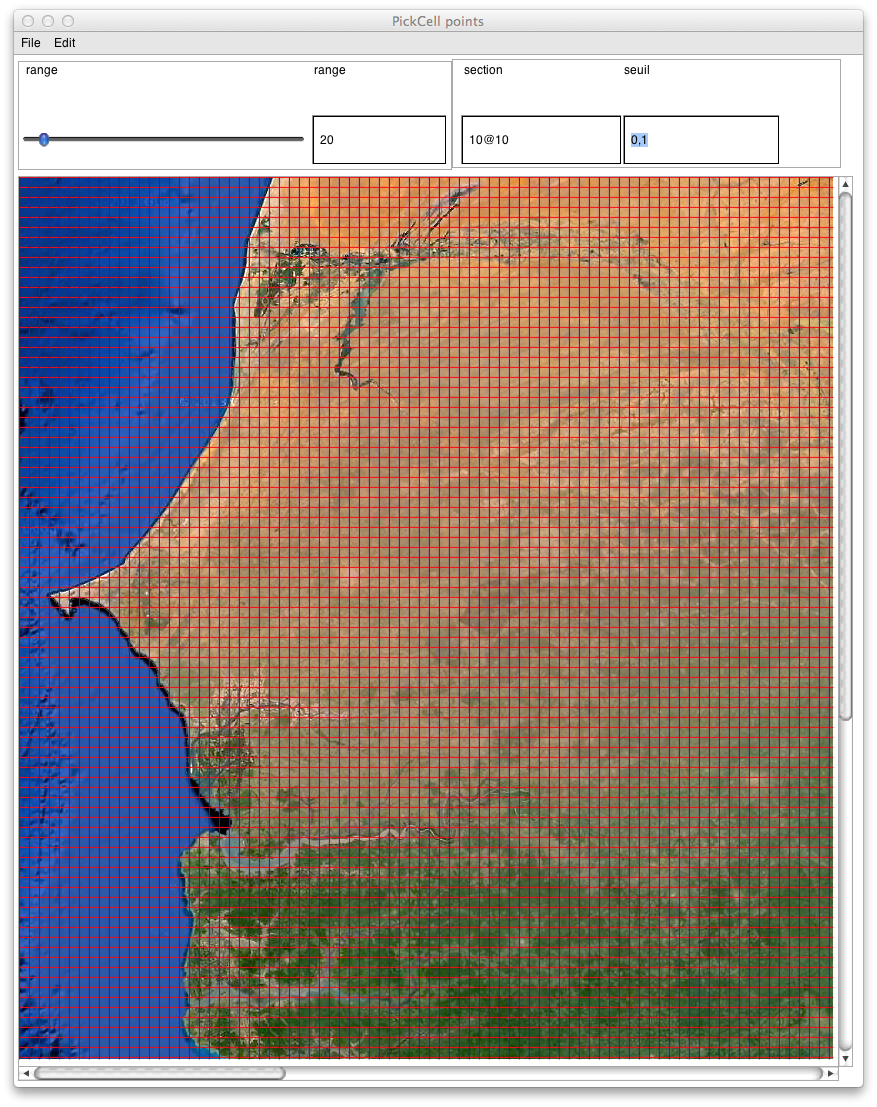
\includegraphics[width=10cm]{SenegalGrid10x10.png}
\caption{Using a 10@10 grid, the image is split into $10\times10$ pixels. 
Following the application, it is possible to specify $x  \times   y$ grids with $x  \neq  y$.}
\label{fig:SenegalGrid10x10}
\end{center}
\end{figure}

Having split the image into cells, it is now possible to classify thems around common properties.

\begin{figure}[hbtp]
\begin{center} 
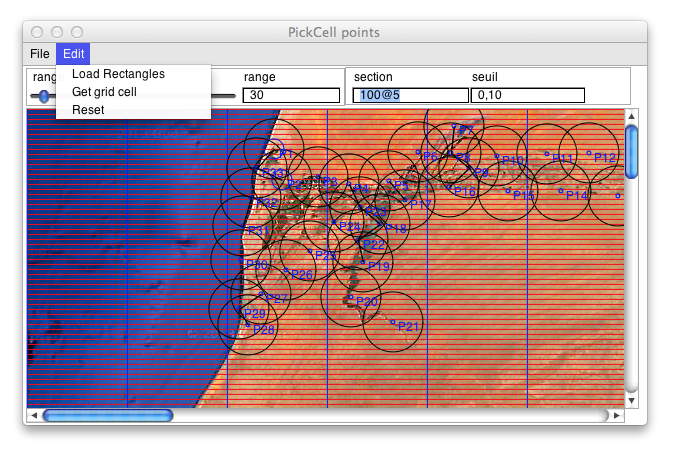
\includegraphics[width=10cm]{SenegalGetGridCell.png}
\caption{Rectangular grid, and sensor geometry specification. The Edit Menu {\sl Get Grid Cell} allows to go a step forward in the flow
to group cell togethers and form {\sl regions} of interest. Section \ref{sec:classification}}
\label{fig:SenegalGetGridCell}
\end{center}
\end{figure}

\subsection { Grouping cells  into classes}
\label{sec:classification} 
\subsubsection { Computing statistics}

From the menu shown Figure  \ref{fig:SenegalGetGridCell}, we obtain a new tool for region
specification and manipulation. As for the grid in segmentation, a new parameter allows to divide
the cell space according to pixel distributions.The choice of group distribution  can be more or less sophisticated.
To start by the begining, the following algorithm is applied to the whole cell grid, to obtain a set of $min, max, mean$ parameters
on each colour :

\begin{lstlisting}  
STEP 1
	for each cell in the grid
		for each pixel in the cell 
			 for each colour component in { R, G, B}
				 update (min(colour))
				 update (max(colour))
				 update (sum(colour))
		 for each colour component in { R, G, B}
			 update (mean(colour))
\end{lstlisting}

Following this step, we have $3 \times 3$ parameters set in each cell, thus allowing to compute
global image characteristics that will reflect the efficiency of the preprocessing:

\begin{lstlisting}  
STEP 2
	for each cell in the grid
		for each colour component in { R, G, B}
			update(minGlobal)
			update(maxGlobal)
			update(minMeanGlobal)
			update(maxMeanGlobal)
\end{lstlisting}


\begin{figure}[hbtp]
\begin{center} 
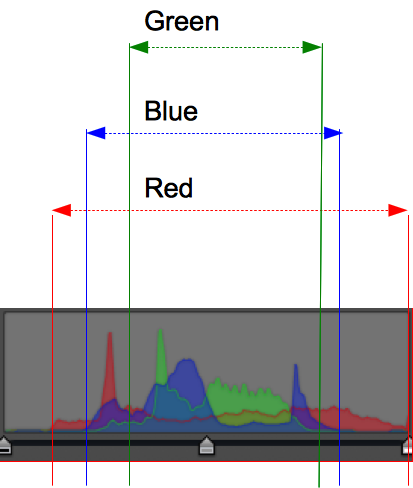
\includegraphics[width=6cm]{RGBDiagram.png}
\caption{From the preprocessing results shown Figure \ref,{fig:colours1+2},   we can guess min(colour), max(colour) for each
component in Red Green Blue.}
\label{fig:RGBDiagram}
\end{center}
\end{figure}

After this step and for each component in RGB space, we have global $[min,max] $ measures for:

\begin{itemize}
\item the value taken over the image (see Figure \ref{fig:RGBDiagram} )
\item the mean of values in each cell
\end{itemize}



\subsubsection { Grouping cell together }

We can use the values computed in each cell and globally to group cell togethers. For the minimum
and the maximum, and even the mean in each cell, a simple algorithm is as follows:

\begin{lstlisting}  
STEP3
	decide on a partition in N>1
	for each component in RGB
		discard any value out side the  [min,max]   interval found for the component
		produce N adjacent sub intervals   [min,max]  
\end{lstlisting}

In the case of $N=2$ the RGB min, max, or mean values in each cell will allow to {\sl classify}
each cell in an unique way in a $2^3$ interval space $(R_0,R_1) \times (G_0,G_1) \times (B_0,B_1) $.
The {\sl cube} of coordinates go from $0,0,0= 0$ to $1,1,1= 7$.
By selecting {\sl Get grid cell} shown Figure \ref{fig:SenegalGetGridCell} the classification tool appears.

What does this too is to allow the selection of $N$, then each cell is tne image is assigned to an interval
depending on its values. By selecting codes as defined above, the corresponding regions appear
an part of the original image. 


\begin{lstlisting}  
STEP4
	for each interval allocate a collection to record cells pertaining to this interval
	for each cell in the grid record the cell in its interval with the geographic position
\end{lstlisting}


\begin{figure}[hbtp]
\begin{center} 
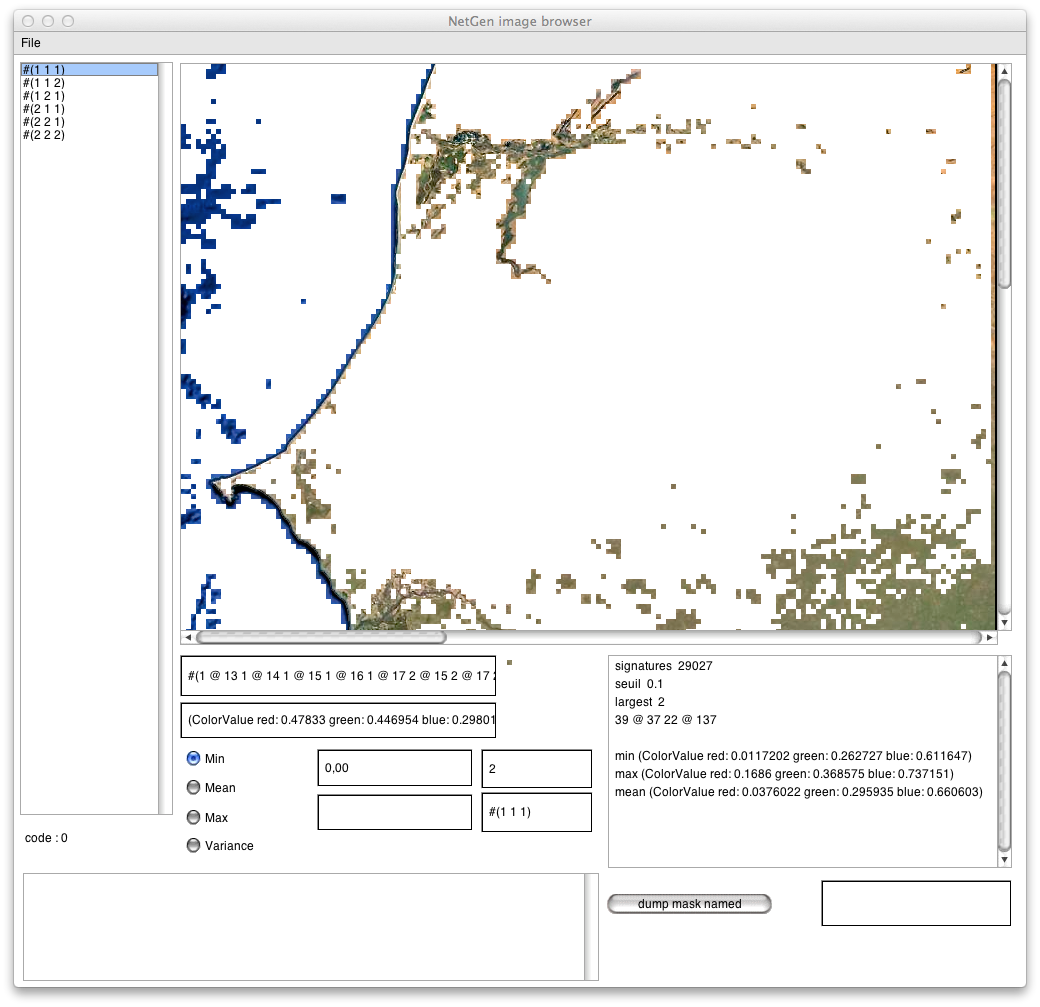
\includegraphics[width=12cm]{Senegal5x5code0.png}
\caption{Pixel class  browser displaying the region corresponding to code 0 : lowes interval in each component of R, G, B.
Shore and rivers appear as dark cell when the minimum criteria are selected. The partition is N=2, code is 0, for (R=1,G=1,B=1).}
\label{fig:Senegal5x5code0}
\end{center}
\end{figure}

\section{Cell system synthesis}
\subsection { Weaving a  network }

Given a cell system produced from a class, grouping several classes, or from a whole image, 
we can now consider to produce a process organization. Taking one node, there are many way to decide
which neighbours are visible, and this task can appear simple if we use a connexion pattern.
Cellular automata use these patterns to define neighborhood.

Examples of neighborhood are Von Neumann cross, or Moore square. Mathematical morphology
methods allow these neighborhood to be arbitrary shapes. As an example two line segments
could figure a plane in the sky.


\begin{figure}[hbtp]
\begin{center} 
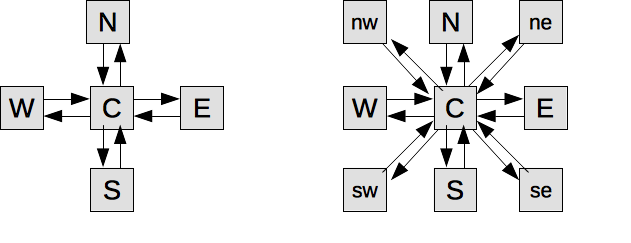
\includegraphics[width=10cm]   {VonNeumann.png}
\caption{Von Neumann and Moore neigborhood with distance = 1}
\label{fig:VonNeumann}
\end{center}
\end{figure}

To build a cell system, the class is swept, row by row, column by column.
For each existing cell, a process is created.

In a second stage,   the class is again swept cell by cell.
For each cell C,   the neighborhood positions  are searched   inside the class.
For each existing neighbour, links are established with the center C.
This way a network of celles is weaved according to the neighborhood
and the class geometric organization. Figure \ref{fig:classBrowser}
displays the Cell class browser with choice of standard neighborhhod at the bottom.




\begin{figure}[hbtp]
\begin{center} 
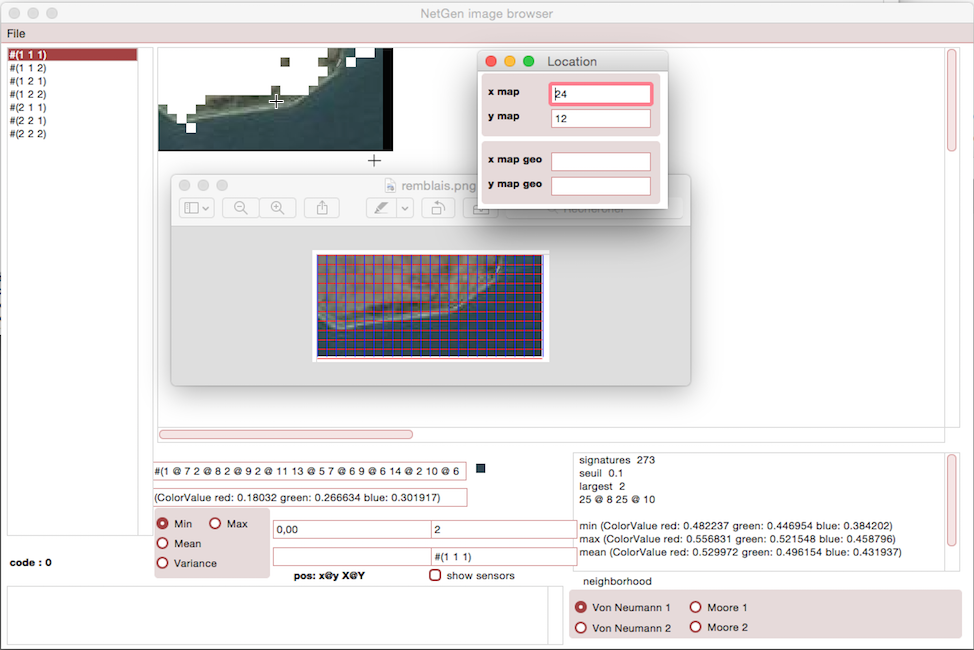
\includegraphics[width=12cm]{classBrows+Loc+mask.png}
\caption{Segmented image and its distribution into classes, code 0 selected.
Picture shows a cross cursor above one of the cell ant the location of the cell.
This cell has neighbours at North, South, East and West, and thus has a full Von Neumann neighborhood.
However a Moore neighborhood would be incomplete due to cells lacking in the north}
\label{fig:classBrowser}
\end{center}
\end{figure}

\begin{figure}[hbtp]
\begin{center} 
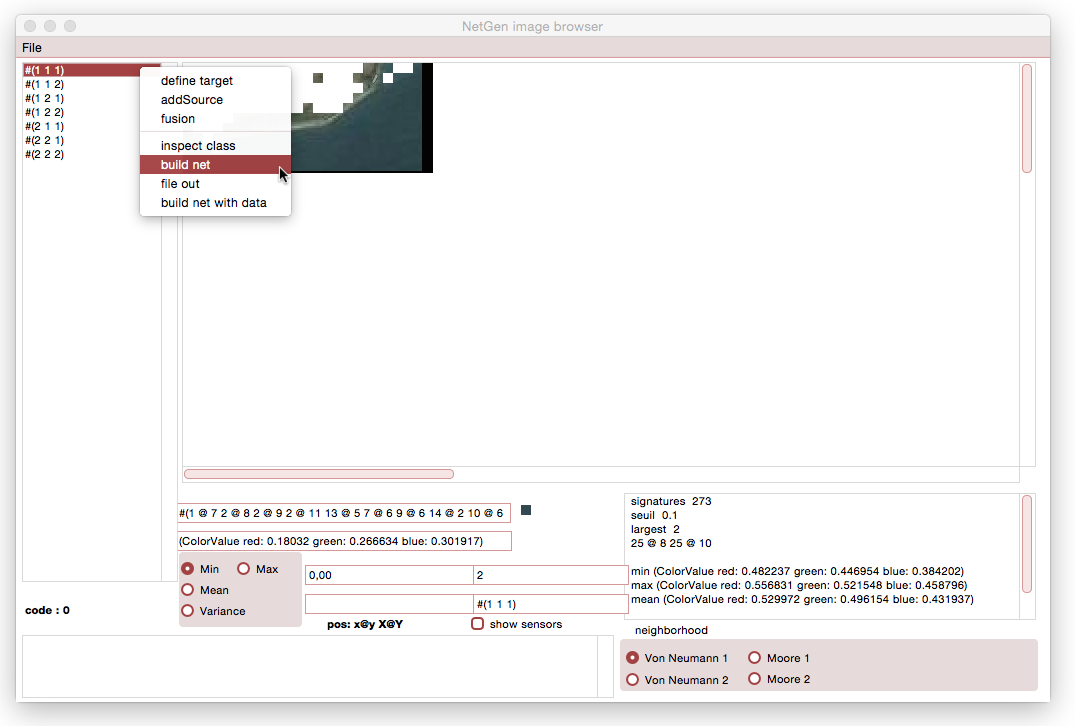
\includegraphics[width=8cm]{generatingCellNetwork.png}
\caption{Calling the network generator on a cell class}
\label{fig:generatingCellNetwork}
\end{center}
\end{figure}
\subsection {Programs generation }

Once the network is built, programs can be produced to represent its process and topology.
Menu in the cell class list has a {\sl Build net} option for this (figure \ref{fig:generatingCellNetwork}.
The results are produced in NetGen windows available as shown figure  \ref{fig:cellNetworkSample}.
There is atmost 4 processes in the fanout for each cell, and isolated process are removed.
The abstract network is described as shown below~:
\begin{lstlisting}
cellNetwork0

messages none  defined. 
Px23y8 { Px22y8, Px23y9, Px24y8, Px23y7 } CellNode (23 @ 8) (20)
Px20y10 { Px20y9, Px20y11, Px21y10, Px19y10 } CellNode (20 @ 10) (20)
Px17y7 { Px17y6, Px16y7, Px17y8, Px18y7 } CellNode (17 @ 7) (20)
Px12y8 { Px12y9, Px12y7, Px13y8, Px11y8 } CellNode (12 @ 8) (20)
...
\end{lstlisting}


In this text, each process is named using its position, as example $Px23y8$ is located at
row 8, columns 23. The name of the procedure executed is CellNode() to distinguish with Node()
used inside sensor networks. Positions and range also appear at the end of the line.


\begin{figure}[hbtp]
\begin{center} 
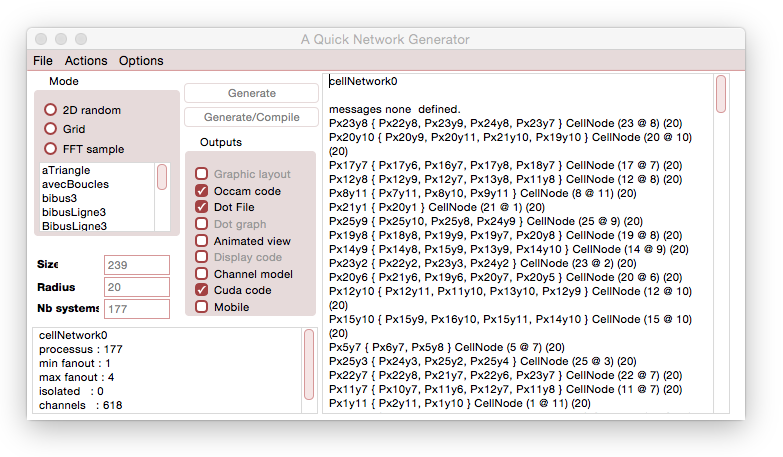
\includegraphics[width=12cm]{cellNetworkSample.png}
\caption{Screencast showing the abstract specification of a generated network for code 0 class.
One process per line, as for sensor networks.}
\label{fig:cellNetworkSample}
\end{center}
\end{figure}

Statistics show that fanout is limited to four, fanin at least equal to 1. There are 177 cells.
Occam (and CUDA) process systems have been produced by the generator that  still need
behaviour description for  their  cella. This behaviour can be very standard transition rule
for cellular automata, but networking behaviuor could apply as well:

\begin{itemize}
\item diameter computation : longest distance between cells,
\item leaders : for naming and differentiating subnetworks
\item routing tables : to reach any cell from any cell in the same network
\item packet transport and delivery, etc\ldots
\end{itemize}

\subsection {Compiling and simulating }

The shortest path to simulate is to reuse a sensor network Occam behaviour file,
as example for leader and diameter dynamic computation. The Actions menu
of NetGen window allows to do it (figure \ref{fig:NetGenAlgo}).

\begin{figure}[hbtp]
\begin{center} 
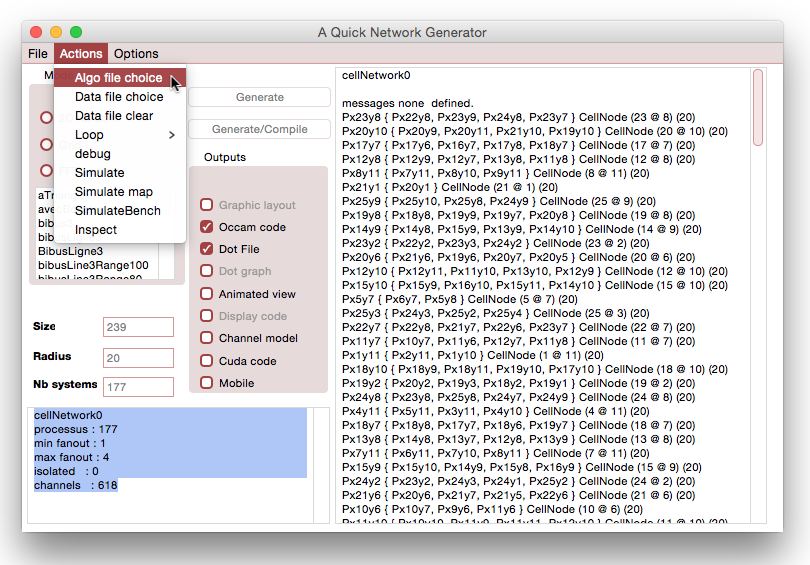
\includegraphics[width=12cm]{NetGenAlgoFile.png}
\caption{Selection of include files: for  behaviour, and also for data files holding the cell contents.}
\label{fig:NetGenAlgo}
\label{fig:includeFiles}
\end{center}
\end{figure}

Once this is done, the action flow is asfollow:
\begin{enumerate}
\item Check coherency between behaviour file and architecture file: in particular the name of the
procedures executed by processes must be the same. For this example, it is CellNode(),
defined in {\sl cellnodes-test-include-diam.occ}.
\item Compile architecture. As example :\\
kroc -lcourse cellNetwork17.occ
\item Check the execution trace.
\end{enumerate}


\section {Physical cell system illustration :  Antsiranana geography capture and analysis }

\begin{figure}[hbtp]
\begin{center} 
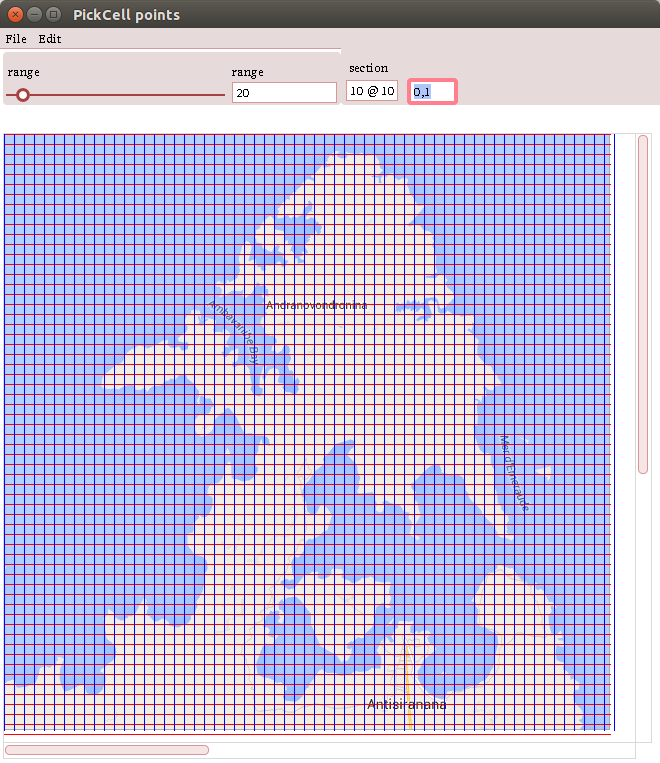
\includegraphics[width=10cm]{diego-split-10x10.png}
\caption{Google map API3 was used to select Antsiranana bay and feed PickCell : $10 \times 10$ pixel cells.}
\label{fif:sampleAntsiranana}
\end{center}
\end{figure}

\subsection {Sample : Antsiranana  cell classification  }

We then select one pixel space and generate networks. and graph for neighborhood VonNeumann 1
The graph seems to present a single network, isn't it?

\begin{figure}[hbtp]
\begin{center} 
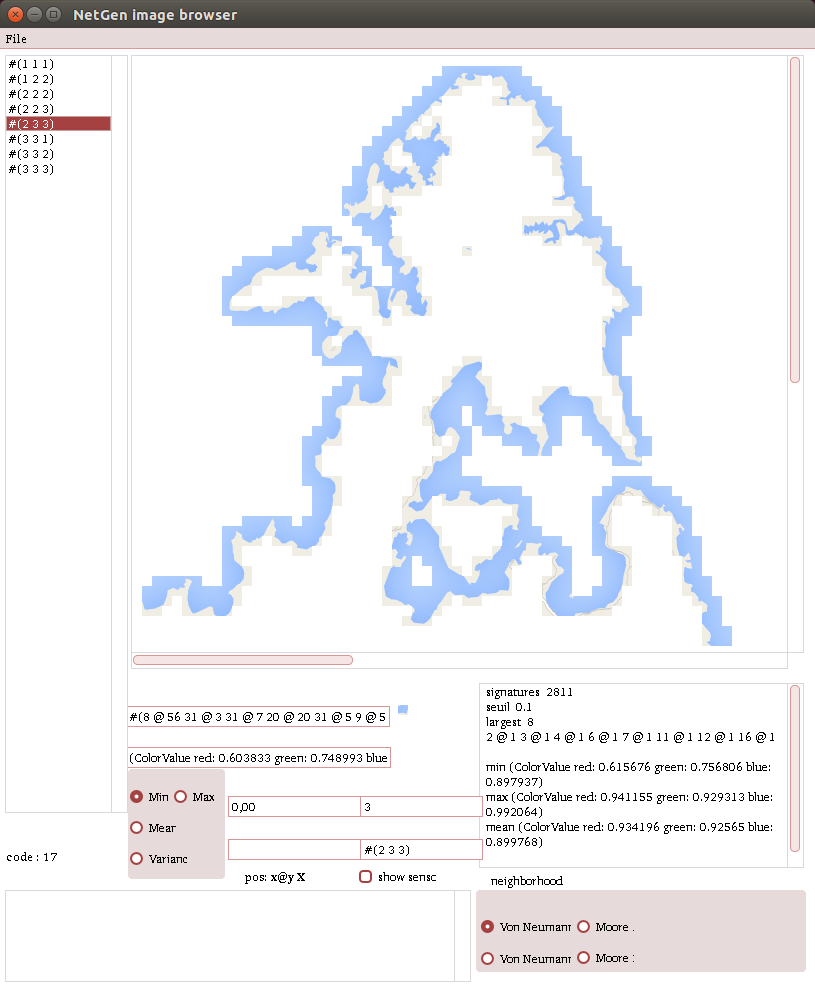
\includegraphics[width=10cm]{diego-class17-3.png}
\caption{The pixel  space was split into 27 subspaces  defining classes.}
\label{fig:antisrananaClass17}
\end{center}
\end{figure}


\begin{figure}[hbtp]
\begin{center} 
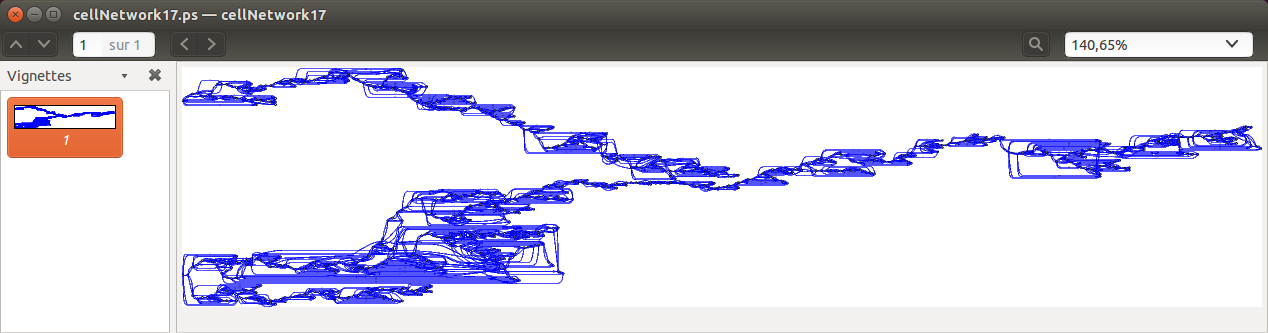
\includegraphics[width=12cm]{diegoGraph17.png}
\caption{Resulting   logic  graph for Von Neumann1 neighborhod.  How many subgraphs  ? see section \ref{sec:comment} }
\label{fig:ansirananaGraph}
\end{center}
\end{figure}

\subsection{ Neighborhood statistics}

The four standatd neighborhood were selected in turns. Statistics came from the NetGen window
after accepting the different network (table \ref{tab:uneCATable}).


\begin{table}[htb]
\begin{center}
\begin{tabular}{|l|l|l|l|l||}\hline
cellNetwork17 & VN1 &   VN2 &   M1 &    M2\\\hline
processus  &    809 &   809 &   809 &   809\\\hline
min fanout  &   1 &     3 &     2 &     6\\\hline
max fanout  &   4 &     12 &    8 &     22\\\hline
isolated    &   0 &     0 &     0 &     0\\\hline
channels    &   2440 &  6346 &  4576 &  10962\\\hline
neighborhood size  &   4 &  12 &  8 &  22\\\hline
\end{tabular}
\caption{ Four different neighborhood generated for Antsiranana bay with distances 1 and 2.
the table show  cell  networks characteristics. }
\label{tab:uneCATable}
\end{center}
\end{table}


\subsection{ Trace and execution }
\label{sec:antsiranan}

Once the program is compiled, we can launch an execution, with more than 800 processes
working together. The program compute the leader Id, and the diameter of network(s).
The trace coming from execution has the following contents:


\begin{lstlisting}
 Id	diam	leader
 784	  84 803
   2	  84 803
   5	  84 803
...
 803	  84 803
 668	 197 808
   0	 197 808
   1	 197 808
...
\end{lstlisting}

\begin{table}[htb]
\begin{center}
\begin{tabular}{|l|l|l|}\hline
identity  & diameter  & leader \\\hline
 784&	  84& 803\\\hline
   2	&  84 &803\\\hline
   5	&  84 &803\\\hline
... & .. & ..\\\hline
 803&	  84& 803\\\hline
 668&	 197& 808\\\hline
   0	& 197& 808\\\hline
   1	& 197& 808\\\hline
... & .. & ..\\\hline
 806	& 197& 808\\\hline
 807	& 197& 808\\\hline
 808	& 197& 808\\\hline
\end{tabular}
\caption{Simulation trace: smallest networks (84-803)  finish first in the case of Occam execution.
It is not the case for CUDA execution. }
\label{tab:uneTableTrace}
\end{center}
\end{table}

Therefore we have two {\sl cell networks } of leaders 803 and 808, and diameters 84 and 197.
Any information circulating in the second network will use at most 197 hops to
reach a destination.

All the algorithms  are not equivalent. See table \ref{tab:uneTableBench} showing a comparison between A and 
running on a multicore i7 CPU. It is noticeable that B has a strong advantage and a higher level
of effective parallelism (see the user row).

\begin{table}[htb]
\begin{center}
\begin{tabular}{|l|l|l|}\hline 
time &  A & B \\\hline
real &  5m24.271s &     0m9.843s\\\hline
user &  5m40.865s &     0m28.074s\\\hline
sys  &  0m0.686s  &     0m0.674s\\\hline
\end{tabular}
\caption{ Two programs A and B executed on the same network. A is for naive
leader and diameter computations. B is for diameter computation saving useless
data transmission. }
\label{tab:uneTableBench}
\end{center}
\end{table}

\section{Neighborhood discovery and isotropy}

As for computer networks,  cellular automata built from analysis have irregularities:

\begin{itemize}
\item shape are  produced from classes, and shapes have frontiers. That means that
if a Von Neumann neighborhood was taken as a connectivity pattern, cells do not have
complete neighborhood.
\item another problem comes from this lack of completion: how can we guess the direction addressed
by a link array ? Which link lead to where ?
\begin{itemize}
\item in the physical world links do not really exist, but direction can be significant,
\item cellular automata can be isotropic, or anisotropic, making directions critical
in transition rules.
\end{itemize}
\end{itemize}




Figure \ref{fig:antisrananaClass17} display a shore obtained from a map system.
As discussed in section \ref{sec:antsiranan} the cell network is distributed into
two parts showing diameters as large as 197 cell paths. If we are to model the effect
of a particular wind on surface tides, we need to know the direction available at each
cell point.

Thus local connectivity discovery is needed. As for sensor networks, it is interesting
to maintain connectivity knowledge  dynamically, and thus, during simulation.

 \subsection {Neighbourhood data structures explained }

The element of Occam coding below allows to see what will append. Basically there
is a descriptor for each detected neighbour. These descriptors will be stored
in a dynamic table, and a redefinition of link protocol allows to pass these tokens
on communication links (abstract, of course).

\begin{lstlisting}  
DATA TYPE KnownNeighbour
  RECORD
    INT Id: -- node identity
    INT linkIndex:  -- index of link
    Location relativeLoc: -- xLoc yLoc record
:
DATA TYPE Neighbourhood
  RECORD
    INT limit: -- to manage table size
    [MaxFanOut] KnownNeighbour knownNeighbour:
:
PROTOCOL diam.proto
  CASE
    null; BYTE
    file; FileOfId
    int; INT
    location; KnownNeighbour -- for neighbour discovery
:
\end{lstlisting}



Initially each cell has its Id and absolute location stored in a KnownNeighbour
record. The problem is to fill the Neighbourhood table with elements coming
from connected cells.



 \subsection {Neighbourhood   discovery }

In our synchronous simulation frame work, this is a single exchange step
followed by the local building of the neighbourhood table.


\begin{lstlisting}
PROC GetNeighbourhood()
  KnownNeighbour me:
  [MaxFanOut] KnownNeighbour them: 
  SEQ
    GetLocation() -- into Location variable loc
    me[Id] := Id  -- Cell Identity
    me[linkIndex] := -1 
    me[relativeLoc] := loc -- absolute location
    PAR
      PAR j=0 FOR SIZE inChan
        inChan[j] ? CASE
          location ; them[j]   -- get tokens from neighbours
            SKIP 
      PAR j=0 FOR SIZE outChan
        outChan[j] ! location ; me -- send our token
    ResetNeighbourhood(myNeighbours)
    SEQ i=0 FOR SIZE inChan
      SEQ
        them[i][linkIndex] := i --recall link index
        AddInNeighbourhood(loc, them[i],myNeighbours)
         -- add a neighbour and translate absolute to relative location
    DumpNeighbourhood(me, myNeighbours, toMux)  -- trace
:
\end{lstlisting}

\subsection {Trace and comment }

This code was added to previous sample, and few lines were extracted.
During the discovery phasis, each node report its identity, its position, then 
the neighborhood table.

The elements extracted all refers to node 482  located at $x= 32, y=53$.
This node has a full VN1 neighborhood with cardinal directions $ N, E, S,  W$
mapped to link $ 3 , 1, 0, 2$. North is relative coordinates $(0,1)$, West is $(-1, 0)$.
The coordinate system see the origin in $(0,0)$ being at top left of an image.

The name of this cell is Px32y53, and its network diameter is 197.
Notice that cell of Id 479 has an incomplete neighbourhood reduced to 3 cells.

\begin{lstlisting}
./cellNetwork17 | grep 482
248 32 54 { 3 0; 0, 1}{ 57 1; 1, 0}{ 245 2; -1, 0}{ 482 3; 0, -1}
306 33 53 { 57 0; 0, 1}{ 380 1; 0, -1}{ 482 2; -1, 0}{ 741 3; 1, 0}
479 31 53 { 245 0; 0, 1}{ 482 1; 1, 0}{ 564 2; 0, -1}
482 32 53 { 248 0; 0, 1}{ 306 1; 1, 0}{ 479 2; -1, 0}{ 575 3; 0, -1}
575 32 52 { 380 0; 1, 0}{ 482 1; 0, 1}{ 564 2; -1, 0}{ 580 3; 0, -1}
482 Px32y53:
482  197
\end{lstlisting}

We can interpret the trace according to table \ref{tab:cardialAndIndex}. and \label{tab:cardialAndIndex479}.
\begin{table}[htb]
\begin{center}
\begin{tabular}{|l|l|l|}\hline
direction & vector & link index \\\hline
N  &  ( 0, -1) &   3 \\\hline
W  &   ( -1 ,  0 ) &   2  \\\hline
S  &  ( 0, 1) & 0   \\\hline
E  &  ( 1, 0 ) &   1 \\\hline
\end{tabular}
\caption{Node 482 relations between link index and cardinal directions. }
\label{tab:cardialAndIndex}
\end{center}
\end{table}


\begin{table}[htb]
\begin{center}
\begin{tabular}{|l|l|l|}\hline
direction & vector & link index \\\hline
N  &  ( 0, -1) &   2 \\\hline 
S  &  ( 0, 1) & 0   \\\hline
E  &  ( 1, 0 ) &   1 \\\hline
\end{tabular}
\caption{Node 479 relations between link index and cardinal directions. Uncomplete VN1 neighbourhood. }
\label{tab:cardialAndIndex479}
\end{center}
\end{table}




\section { Accessing cell data}

How we can obtain access to cell data produced during image analysis. Look inside
the data file produced as shown figure s \ref{fig:NetGenAlgo} and \ref{fig:generatingCellNetwork}.

\subsection {Data structures }

The data structure appearing in top of the data file are as follows:
\begin{lstlisting}
DATA TYPE ImageExtent -- cell dimension
  RECORD
    INT width:
    INT height:
:
DATA TYPE CellPosition
  RECORD
    INT x:
    INT y:
:
DATA TYPE RGBPixel -- RGB pixel
  RECORD
    BYTE red, green, blue:
:
-- generated description of one cell, size hard coded
DATA TYPE Depth24ByteArray  IS [ 100] RGBPixel:
-- this is a cell image contents with dimensions and contents
DATA TYPE CellImage
  RECORD
    ImageExtent  extent:
    Depth24ByteArray pixelArray:
:
-- this is a complete cell, with its position and data
DATA TYPE CellArray
  RECORD
    CellPosition position:
    CellImage image:
:
-- this is data for one class, 810 cells for this one
VAL [   810] CellArray  Cells IS  -- follows a table of cell contents
-- pages of values
\end{lstlisting}


\subsection {From cell data to cellular automata local state }

(to be continued)






\section { Comments}

\begin{figure}[hbtp]
\begin{center} 
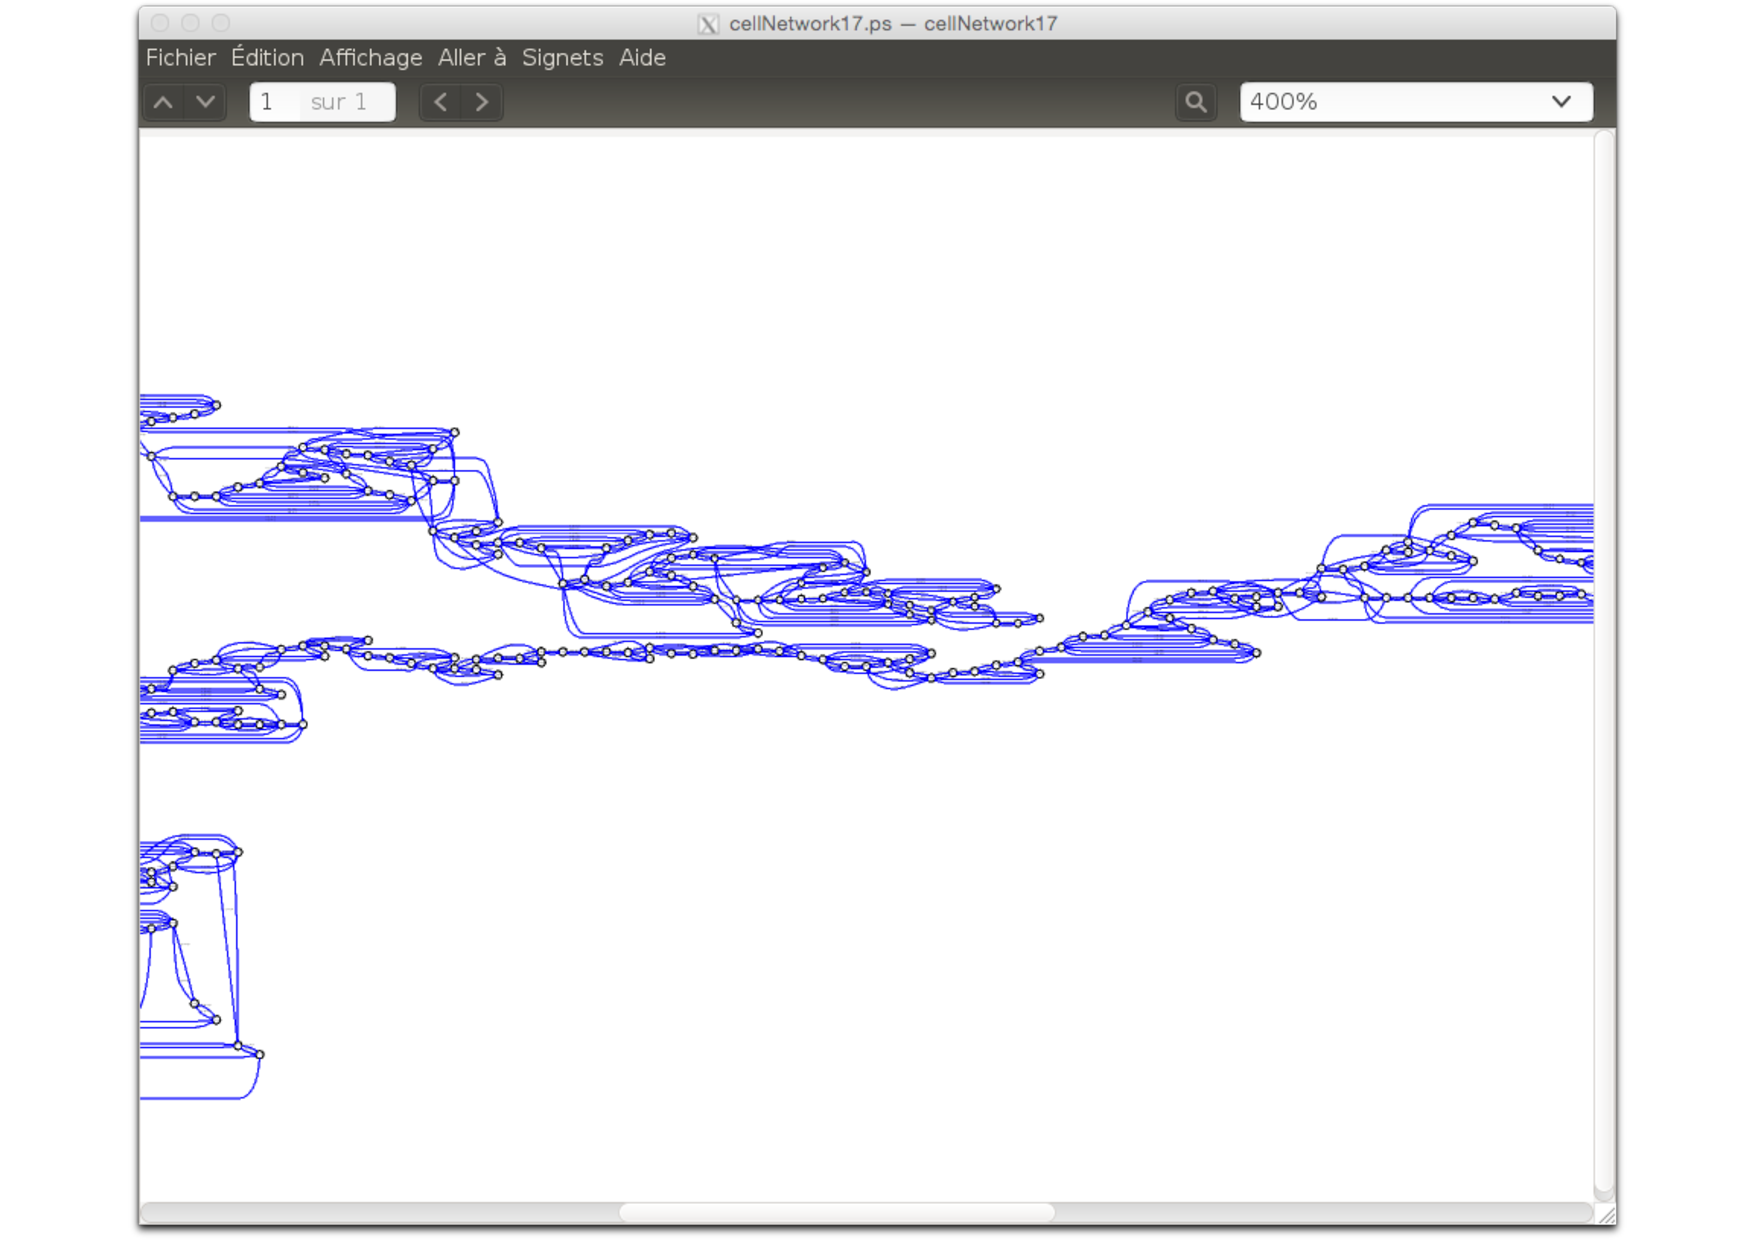
\includegraphics[width=12cm]{Diego2Networks.pdf}
\caption{View on the logic graph..}
\label{fig:antisrananaClass17bis}
\end{center}
\end{figure}

